\documentclass{article}
\usepackage[utf8]{inputenc}

\title{EE2703: Assignment 5}
\author{Yogesh Agarwala \\ EE19B130}
\date{March 25, 2021}

\usepackage{natbib}
\usepackage{graphicx}
\usepackage{amsmath}
\usepackage{listings}

\begin{document}

\maketitle

\section{Introduction}
A wire is soldered to the middle of a copper plate and its voltage is held at 1 Volt. One side of the plate is
grounded, while the remaining are floating. The plate is 1 cm by 1 cm in size.
As a result, current flows. The current at each
point can be described by a “current density” $\vec{j}$. \\\\
This
current density is related to the local Electric Field by the conductivity:


\begin{equation}
    \vec{j} = \sigma\vec{E}
\end{equation}
\\
Electric field is the gradient of the potential:
\begin{equation}
	\vec{E} = - \nabla \phi
\end{equation}
\\
The Continuity Equation:
\begin{equation}
	\nabla \cdot \vec{j} = - \frac{\partial\rho}{\partial t}
\end{equation}
\\
Combining these equations we obtain:

\begin{equation}
    \nabla^2 \phi =  \frac{1}{\rho}\frac{\partial\rho}{\partial t}
\end{equation}
\\
For DC currents, the right side is zero, and we obtain:
\begin{equation}
    \nabla^2 \phi =  0
\end{equation}

\clearpage

\section{Assignment}
\subsection{Taking arguments through commandline}



\lstset{language=Python}
\lstset{frame=lines}
\lstset{label={lst:code_direct}}
\lstset{basicstyle=\footnotesize}
\begin{lstlisting}
if(len(sys.argv)==5):
    Nx, Ny, radius, Niter = [int(x) for x in sys.argv[1:5]]

#default arguments
else:
    Nx = 25
    Ny = 25
    radius = 8
    Niter = 1500
\end{lstlisting}

\subsection{Allocating the potential array and initializing it}
We start by creating an zero 2-D array of size Nx x Ny. then a list of coordinates lying within the radius is generated and these points are initialized to 1.
\begin{lstlisting}
phi = np.zeros((Nx,Ny),dtype = float)
x = np.linspace(-0.5,0.5,num=Nx,dtype=float)
y = np.linspace(-0.5,0.5,num=Ny,dtype=float)
Y,X = np.meshgrid(y,x,sparse=False)
phi[np.where(X**2+Y**2<(0.35)**2)]=1.0

ii = np.where(X**2+Y**2<(0.35)**2)
phi[ii] = 1.0
\end{lstlisting}
\begin{figure}[h!]
\centering
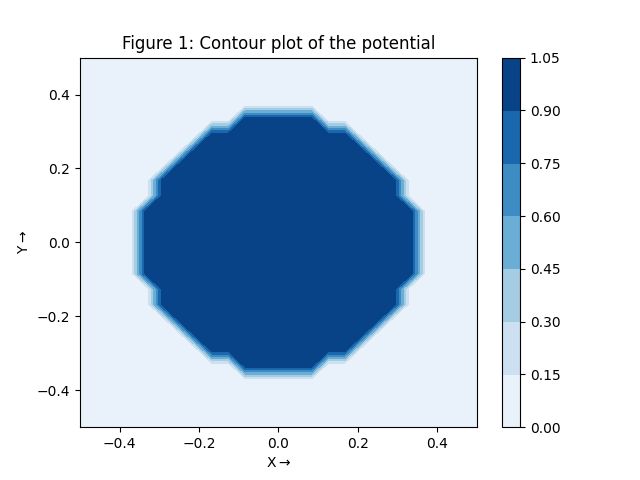
\includegraphics[scale=0.6]{1}
\caption{Contour Plot of the Potential}
\label{fig: Contour Plot of the Potential}
\end{figure}


\subsection{Performing Iterations}

To update the potential we need to first convert it to a difference equation as all of our code is in discrete domain. Thus this is written as:
\begin{equation*}
    \phi_{i,j} = 0.25*(\phi_{i-1,j} + \phi_{i+1,j} + \phi_{i,j+1} + \phi_{i,j-1})
\end{equation*}


\begin{lstlisting}
err = np.zeros(Niter,dtype = float)
for k in range(Niter):
    oldphi = phi.copy()
    
    #updating potential
    phi[1:-1,1:-1] = 0.25*(phi[1:-1,0:-2] + phi[1:-1,2:] + phi[0:-2,1:-1] + phi[2:,1:-1])
    
    #applying boudary conditions
    phi[:,0]=phi[:,1]
    phi[:,Nx-1]=phi[:,Nx-2]
    phi[0,:]=phi[1,:]
    phi[Ny-1,:]=0
    
    phi[ii]=1.0
    err[k] = np.max(np.abs(phi-oldphi))


\end{lstlisting}

\subsection{Plotting the errors}
Note that the error falls very slowly and so it is discouraged to use this method for solving the Laplace equation.
\begin{figure}[h!]
\centering
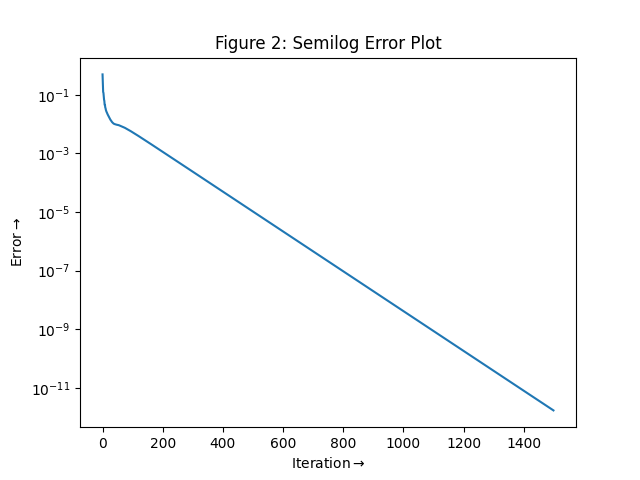
\includegraphics[scale=0.62]{2}
\caption{Semilog Error Plot}
\label{fig:Semilog Error Plot}
\end{figure}
\begin{figure}[h!]
\centering
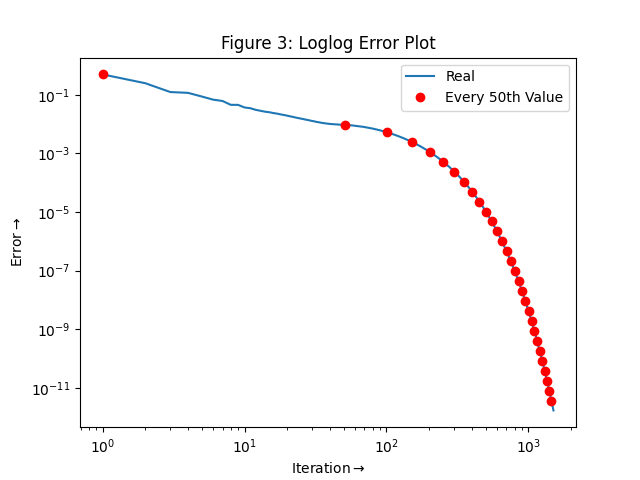
\includegraphics[scale=0.6]{3}
\caption{Loglog Error Plot}
\label{fig:loglog plot of error}
\end{figure}


\subsection{Fitting the error}
Fit1 is drawn by considering all the iterations and Fit2 is drawn without considering the first 500 iterations. There is very little difference between the two fits.


\begin{figure}[h!]
\centering
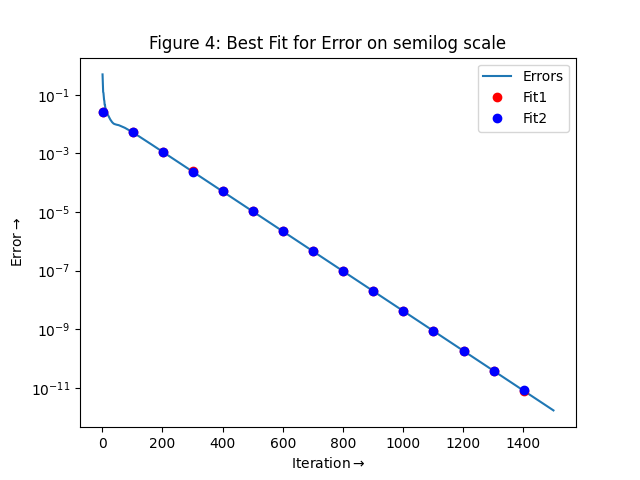
\includegraphics[scale=0.6]{4}
\caption{Best Fit for Error in Semilog scale}
\label{fig:Best Fit of error}
\end{figure}
\begin{figure}[h!]
\centering
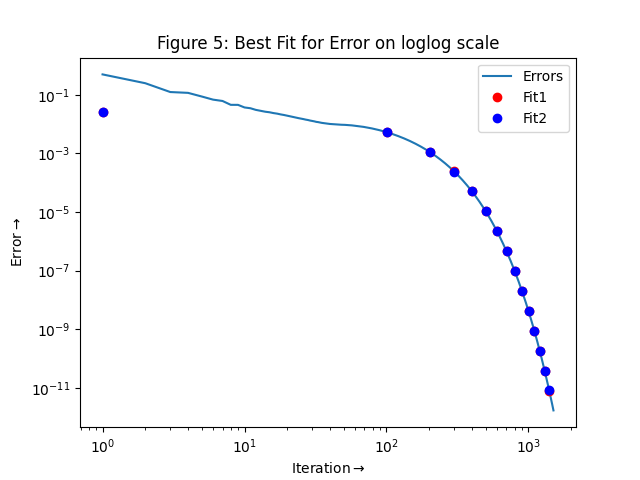
\includegraphics[scale=0.55]{5}
\caption{Best Fit for Error in loglog scale}
\label{fig:Best Fit of error}
\end{figure}

\subsection{Plotting Maximum Possible Error}
\begin{lstlisting}
def NetError(a,b,Niter):
    return -a/b*np.exp(b*(Niter+0.5))
\end{lstlisting}

\begin{figure}[h!]
\centering
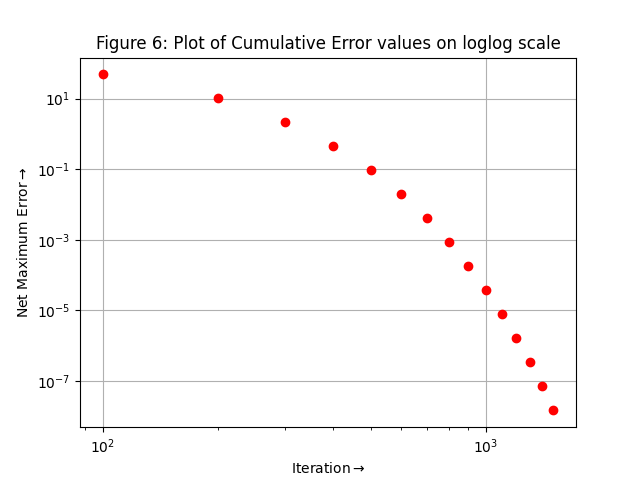
\includegraphics[scale=0.55]{6}
\caption{Cumulative error values on a loglog scale}
\label{fig:3d Plot of Potential}
\end{figure}

\clearpage

\subsection{Surface Plot of Potential}
\begin{lstlisting}
fig1=plt.figure(4)
ax=p3.Axes3D(fig1)
surf = ax.plot_surface(Y, X, phi.T, rstride=1, cstride=1, cmap=plt.cm.jet)
plt.show()
\end{lstlisting}

\begin{figure}[h!]
\centering
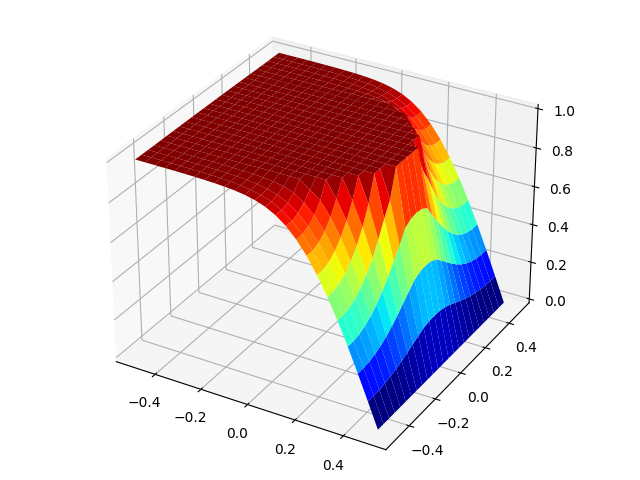
\includegraphics[scale=0.4]{7}
\caption{Surface Plot of Potential}
\label{fig:3D Surface Plot of Potential}
\end{figure}



\subsection{Contour Plot of the Potential}
\begin{lstlisting}
x_c,y_c=np.where(X**2+Y**2<(0.35)**2)
plt.plot((x_c-Nx/2)/Nx,(y_c-Ny/2)/Ny,'ro')
plt.contourf(Y,X[::-1],phi)
plt.show()
\end{lstlisting}

\begin{figure}[h!]
\centering
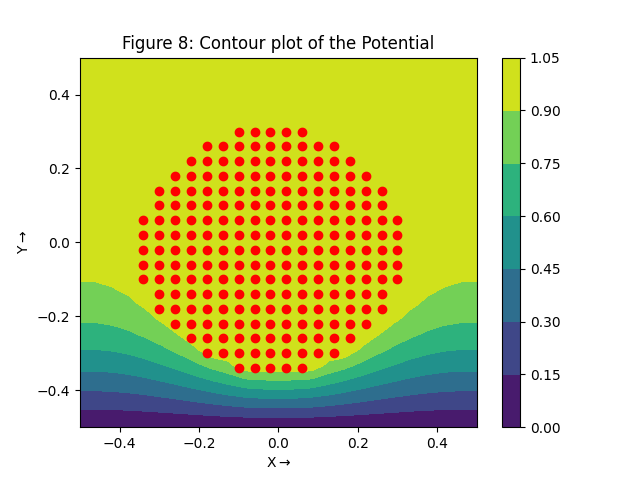
\includegraphics[scale=0.4]{8}
\caption{Contour Plot of the Potential}
\label{fig:2D Contour Plot of the Potential}
\end{figure}
\clearpage
\subsection{Vector Plot of Currents}
Now we obtain the currents. This requires computing the gradient. The actual value of $\sigma$ does not matter to
the shape of the current profile, so we set it to unity. Our equations are
\begin{equation*}
    J_{x,ij} = \frac{1}{2}(\phi_{i,j-1} - \phi_{i,j+1})
\end{equation*}
\begin{equation*}
    J_{y,ij} = \frac{1}{2}(\phi_{i-1,j} - \phi_{i+1,j})
\end{equation*}
\begin{lstlisting}
plt.quiver(Y[1:-1,1:-1],-X[1:-1,1:-1],-Jx[:,::-1],-Jy)
x_c,y_c=np.where(X**2+Y**2<(0.35)**2)
plt.plot((x_c-Nx/2)/Nx,(y_c-Ny/2)/Ny,'ro')
plt.show()

\end{lstlisting}
\begin{figure}[h!]
\centering
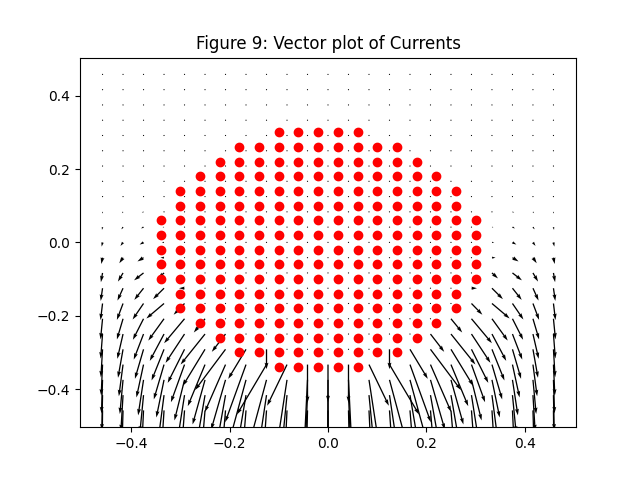
\includegraphics[scale=0.6]{9}
\caption{Vector plot of Currents}
\label{Vector plot of current flow}
\end{figure}


\section{Conclusion}
Using finite differentiation approximation we have found a solution to the
Laplace’s equation for a given system. The error is seen to decay at a
highly gradual pace. Thus the chosen method of solving Laplace’s equation
is inefficient. On analysing the quiver plot of the currents, it was noticed
that the current was mostly restricted to the bottom of the wire, and was
perpendicular to the surface of the electrode and the conductor.

\end{document}
